% !TeX root = ../report.tex
% !TeX spellcheck = en-US
% !TeX encoding = UTF-8
\chapter{DESIGN VALIDATION}\label{chap:design validation}

It is important to validate the performance of the proposed controller, this could either be done in a field test,
full-scale or scaled down, or in a virtual simulation environment. Provided that the simulated environment is an
accurate representation of the physical world. The crawler which was available at the beginning of the project was
unfortunately halfway the project, disassembled and no longer a viable method to verify the proposed controller. Roughly
around the same time, the working environment and contract of of the author changed as well. This forced validation to
be performed in a simulation. This chapter will described the simulation setup and used methods in
Section~\ref{sec:simulation}. The  results are discussed in Section~\ref{sec:results}.

\section{SIMULATION}\label{sec:simulation}
In order to tell something meaningful about performance of a controller, it has to be subject to the same physical
processes, as it would in real-life, albeit in virtual form. Section\ref{sec:motion model} lists assumed forces
and processes acting upon on a crawler and states that drive-train characteristic and soil dynamics play a huge part in
the kinematic behavior of a crawler. There are a couple of physics simulation engines that could be possible candidates
for usage in this project; These are Gazebo, Project Chrono, Bullet and PhyhsX.

From this list, only Project Chrono has an existing framework which takes into account soil dynamic behavior. This can
be simulated using a granular approach, were each particle of sand is body and is modeled using spherical rigid bodies
whose orientation is captured by Euler parameters. For each time step a complete geometric characterization of all
contacting particles is then obtained using collision detection and inter- particle normal contact forces are calculated
by allowing small inter-penetrations using a penalty method for \gls[first]{acr-DEM}. Were the normal contact force is
based on Hertz law and friction forces are calculated using the Coulomb
limit~\cite{recuero_high-fidelity_2017}\cite{serban_co-simulation_2018}. This method is computational heavy and more
suitable for detailed modeling.

An alternative method is \gls[first]{acr-SCM}, based upon the familiar Becker-Wong model. The model provides a
semi-empirical approach to the simulation of soft soil. It offers high speed of simulation and it is accurate enough for
many scenarios. It has the following attributes: it depends on few parameters (the same that are used in the Bekker-
Wong model); it can generate 3D ruts on terrains of variable height; it takes into account multi-pass hardening when
wheels generate intersecting ruts; it can work with irregular triangle-based terrain meshes; it supports an optional
refinement of the terrain mesh to capture fine details like tire threads and lugs; and, it is compatible with deformable
tires and generic shapes like obstacles, track shoes of tanks, etc. On the downside, the new soil model cannot simulate
lateral bulldozing effects like those happening when a tracked vehicle steers in-place and pushes material apart~
\cite{tasora_overview_2018}. This means that the proposed slip-prediction method can't be used in this simulation.

A big part of the physics engine, Project Chrono, is the autonomous vehicle support. This is set-up according to well
known \gls[first]{acr-OOP} practices such as, polymorphism, using virtual overrides in classes that represent physical
bodies. A custom model for different models of a drive-train, body, wheels/tracks and controller can defined and
connected as needed. Were the behavior of that individual model can be thought of as black box. As long as the interface
with the components it connects to are maintained. Section~\ref{sec:simulation model} describes the modeling of the
drive train in detail. The support of realistic sensor characteristic are not yet implemented in Project Chrono, since a
big part of the validation is measuring the performance of a Kalman Filter. An extension for Project Chrono was written,
which allows for the modeling of sensor behavior. This is extension is described in Section~\ref{sec:sensor
simulation}.

\subsection{SENSOR SIMULATION}\label{sec:sensor simulation}

% Describe the lack of sensor simulation and the need to build one

\subsection{SIMULATION MODEL}\label{sec:simulation model}

In this section a model describing the movement of a crawler is outlined. Which allows for an accurate estimate of a
predicted location and orientation of a crawler. The challenge lies in limiting uncertainties, such that path
planning algorithms can be executed without unacceptable drift of a crawler during operations.
%
% \newpage
% \begin{figure}[H]
% 	\begin{center}
% 		\begin{tikzpicture}[auto, node distance=2.5cm,>=latex', align=center]
% 		% Placing the blocks
% 		\node [input, name=input] {};
% 		\node [block, below of=input] (Emotor) {$ E_{motor} $};
% 		\node [left of=Emotor] (formEmotor) {\footnotesize{ $ \left. M_{em} = \frac{p}{\omega} \right\} $}};
% 		\node [sum, below of=Emotor, yshift=-0.5cm, align=center] (sum1) {$ + $ \\ $ - $};
% 		\node [block, right of=sum1, xshift=1cm] (deltaEmotor_Hpump) {$ \int\frac{\Delta \gls{s:tau}}{\gls{s:I}} dt$};
% 		\node [block, below of=sum1] (Hpump) {$ H_{pump} $};
% 		\node [left of=Hpump, xshift=-2cm] (formHpump) {\footnotesize{ $\arraycolsep=1.4pt\def\arraystretch{1} \left. \begin{array}{r}
% 			\gls{s:hydraulic flow} = \gls{s:v_f} \gls{s:A_p} \\
% 			\gls{s:hydraulic flow} = \gls{s:ideal hydraulic flow} - \gls{s:leak hydraulic flow} \\
% 			\gls{s:tau} = \gls{s:tau_ideal} + \gls{s:tau_friction} \\
% 			\gls{s:ideal hydraulic flow} = D \omega \\
% 			\gls{s:tau_ideal} = D \Delta p \\
% 			\gls{s:leak hydraulic flow} = K_{HP} \Delta p \\
% 			\tau_{friction} = \left(\tau_{0} + K_{TP}|\Delta P|\right) \text{tanh}\left(\frac{4 \omega}{\omega_{thresh}} \right) \\
% 			K_{HP} = \frac{\mathsf{v}_{Nom}}{\rho \mathsf{v}} \frac{\rho_{Nom} \omega_{Nom} D}{\Delta p_{Nom}} \left(1 - \eta_{V,Nom}\right)
% 			\end{array} \right\} $ }};
% 		\node [sum, below of=Hpump, yshift=-0.5cm, align=center] (sum2) {$ + $ \\ $ - $};
% 		\node [block, right of=sum2, xshift=1cm] (deltaHpump_Emotor) {$ \int\frac{\Delta p A_{p}}{m_{f}} dt$};
% 		\node [block, below of=sum2] (Hmotor) {$ H_{motor} $};
% 		\node [sum, below of=Hmotor, yshift=-0.5cm, align=center] (sum3) {$ + $ \\ $ - $};
% 		\node [left of=Hmotor, xshift=-2cm] (formHmotor) { \footnotesize{ $\arraycolsep=1.4pt\def\arraystretch{1} \left. \begin{array}{r}
% 			\gls{s:hydraulic flow} = \gls{s:v_f} \gls{s:A_p} \\
% 			\gls{s:hydraulic flow} = \gls{s:ideal hydraulic flow} + \gls{s:leak hydraulic flow} \\
% 			\gls{s:tau} = \gls{s:tau_ideal} - \gls{s:tau_friction} \\
% 			q_{ideal} = D \omega \\
% 			\gls{s:tau_ideal} = D \Delta p \\
% 			q_{leak} = K_{HP} \Delta p \\
% 			\tau_{friction} = \left(\tau_{0} + K_{TP}|\Delta P|\right) \text{tanh}\left(\frac{4 \omega}{\omega_{thresh}} \right) \\
% 			K_{HP} = \frac{\mathsf{v}_{Nom}}{\rho \mathsf{v}} \frac{\rho_{Nom} \omega_{Nom} D}{\Delta p_{Nom}} \left(\frac{1}{\eta_{V,Nom}} - 1\right)
% 			\end{array} \right\} $ }};
% 		\node [block, right of=sum3, xshift=1cm] (deltaHmotor_Propulsion) {$ \int\frac{\Delta \tau}{I} dt$};
% 		\node [block, below of=sum3] (Propulsion) {$ Propulsion $};
% 		\node [left of=Propulsion, xshift=-2cm] (formHmotor) { \footnotesize{ $\arraycolsep=1.4pt\def\arraystretch{1} \left. \begin{array}{r}
% 			\gls{s:gamma_sw} = \gls{s:g} (\gls{s:rho_s} - \gls{s:rho_w}) \\
% 			\gls{s:n} = \gls{s:gamma_sw} \frac{(2\gls{s:R_a})^2}{\gls{s:d_a}}\sin(\gls{s:theta_s}-\gls{s:theta_s}\cos(\gls{s:theta_s})) \\
% 			\gls{s:n} = \gls{s:p} = \gls{s:s_c} \gls{s:c} \gls{s:N_c} + \gls{s:s_q} \gls{s:q} \gls{s:N_q} + \gls{s:s_gamma} \frac{1}{2} \gls{s:gamma_sw} \gls{s:W_a} \gls{s:N_gamma} \\
% 			\gls{s:N_q} = \frac{1 + \sin \gls{s:phi_s}}{1 - \sin \gls{s:phi_s}} \exp(\pi \tan \gls{s:phi_s}) \\
% 			\gls{s:N_c} = (\gls{s:N_q} - 1)\cot \gls{s:phi_s} \\
% 			\gls{s:N_gamma} = 2(\gls{s:N_q} - 1)\tan \gls{s:phi_s} \\
% 			\gls{s:s_q} = 1 + \frac{\gls{s:W_a}}{\gls{s:l_a}} \sin \gls{s:phi_s} \\
% 			\gls{s:s_c} = 1 + 0.2 \frac{\gls{s:W_a}}{\gls{s:l_a}} \\
% 			\gls{s:s_gamma} = 1 - 0.3 \frac{\gls{s:W_a}}{\gls{s:l_a}} \\
% 			\gls{s:V_sa} = \gls{s:A_s} \gls{s:l_a} \\
% 			\gls{s:A_s} = \pi \gls{s:R_a}^2(\gls{s:theta_s} - \sin(\gls{s:theta_s})\cos(\gls{s:theta_s})) \\
% 			\gls{s:s_a} = \gls{s:R_a} \gls{s:theta_s} \\
% 			\gls{s:d_a} = \gls{s:R_a}\left(1-\cos(\frac{\gls{s:theta_s}}{2})\right) \\
% 			\gls{s:F_b} = g \gls{s:V_sa} \left(\rho_s - \rho_w\right)
%
% 			\end{array} \right\} $} };
% 		\node [sum, below of=Propulsion, yshift=-0.5cm, align=center] (sum4) {$ + $ \\ $ - $};
% 		\node [block, right of=sum4, xshift=1cm] (deltaForce) {$ \int\frac{\Delta F}{m_{adb}} dt$};
% 		\node [block, below of=sum4] (Resistance) { $ F_{resistance} $ };
%
% 		\node [input, right of=deltaEmotor_Hpump] (p1) {};
% 		\node [input, above of=p1, yshift=-2.5mm] (p1a) {};
% 		\node [input, below of=p1, yshift=2.5mm] (p1b) {};
%
% 		\node [input, right of=deltaHpump_Emotor] (p2) {};
% 		\node [input, above of=p2, yshift=-2.5mm] (p2a) {};
% 		\node [input, below of=p2, yshift=2.5mm] (p2b) {};
%
% 		\node [input, right of=deltaHmotor_Propulsion] (p3) {};
% 		\node [input, above of=p3, yshift=-2.5mm] (p3a) {};
% 		\node [input, below of=p3, yshift=2.5mm] (p3b) {};
%
% 		\node [input, right of=deltaForce] (p4) {};
% 		\node [input, above of=p4, yshift=-2.5mm] (p4a) {};
% 		\node [input, below of=p4, yshift=2.5mm] (p4b) {};
%
% 		\node [right of=p4, xshift=-10mm] (output) {Dredgebot \\ speed};
%
% 		\draw [draw,->] (input) -- node [left] {$p $ \\ $ [W] $} (Emotor);
% 		\draw [->] (Emotor) -- node [left] {$ \tau $ \\ $ [Nm] $} (sum1);
% 		\draw [->] (Hpump) -- node [left] {$ \tau $ \\ $ [Nm] $} (sum1);
% 		\draw [->] (sum1) -- node {$ \Delta \tau $ \\ $ [Nm] $} (deltaEmotor_Hpump);
% 		\draw [-] (deltaEmotor_Hpump) -- node {$ \omega $ \\ $ [rad/s] $} (p1);
% 		\draw [-] (p1) -- (p1a);
% 		\draw [->] (p1a) -- ($ (Emotor.east)+(0,-0.25) $);
% 		\draw [-] (p1) -- (p1b);
% 		\draw [->] (p1b) -- ($ (Hpump.east)+(0,0.25) $);
%
% 		\draw [->] (Hpump) -- node [left] {$ p $ \\ $ [Pa] $} (sum2);
% 		\draw [->] (Hmotor) -- node [left] {$ p $ \\ $ [Pa] $} (sum2);
% 		\draw [->] (sum2) -- node {$ \Delta p $ \\ $ [Pa] $} (deltaHpump_Emotor);
% 		\draw [-] (deltaHpump_Emotor) -- node {$ v $ \\ $ [m/s] $} (p2);
% 		\draw [-] (p2) -- (p2a);
% 		\draw [->] (p2a) -- ($ (Hpump.east)+(0,-0.25) $);
% 		\draw [-] (p2) -- (p2b);
% 		\draw [->] (p2b) -- ($ (Hmotor.east)+(0,0.25) $);
%
% 		\draw [->] (Hmotor) -- node [left] {$ \tau $ \\ $ [Nm] $} (sum3);
% 		\draw [->] (Propulsion) -- node [left] {$ \tau $ \\ $ [Nm] $} (sum3);
% 		\draw [->] (sum3) -- node {$ \Delta \tau $ \\ $ [Nm] $} (deltaHmotor_Propulsion);
% 		\draw [-] (deltaHmotor_Propulsion) -- node {$ \omega $ \\ $ [rad/s] $} (p3);
% 		\draw [-] (p3) -- (p3a);
% 		\draw [->] (p3a) -- ($ (Hmotor.east)+(0,-0.25) $);
% 		\draw [-] (p3) -- (p3b);
% 		\draw [->] (p3b) -- ($ (Propulsion.east)+(0,0.25) $);
%
% 		\draw [->] (Propulsion) -- node [left] {$ F $ \\ $ [N] $} (sum4);
% 		\draw [->] (Resistance) -- node [left] {$ F $ \\ $ [N] $} (sum4);
% 		\draw [->] (sum4) -- node {$ \Delta F $ \\ $ [N] $} (deltaForce);
% 		\draw [-] (deltaForce) -- node {$ v $ \\ $ [m/s] $} (p4);
% 		\draw [-] (p4) -- (p4a);
% 		\draw [->] (p4a) -- ($ (Propulsion.east)+(0,-0.25) $);
% 		\draw [-] (p4) -- (p4b);
% 		\draw [->] (p4b) -- ($ (Resistance.east)+(0,0.25) $);
% 		\draw [->]	(p4) -- (output);
% 		%\draw [->] (y) |- (measurements);
% 		%\draw [->] (measurements) -| node[pos=0.99] {$-$}
% 		%node [near end] {$y_m$} (sum);
% 		\end{tikzpicture}
% 	\end{center}
% 	\caption{Schematic diagram of the propulsion discrete model, based on first-principle}\label{fig:propulsionsystemsimulinkmodel}
% \end{figure}
%
% \subsubsection{Modelling the propulsion system}
% The propulsion system is modelled and shown in \ref{fig:propulsionsystemsimulinkmodel}. In this situation, an electrical motor, drives a hydraulic pump. This electrical motor delivers a certain torque $ \tau $, where the hydraulic pump demands a certain torque. This torque difference $ \Delta \tau $ divided by the sum of inertias and integrated over time, translates to a certain rotational speed $ \omega $, with which this system turns. This hydraulic pump generates a pressure $ p $, with delivers energy to a hydraulic motor, which has a pressure drop, or in other words converts this energy in a certain torque at a certain rotational speed. The pressure difference $ \Delta p $, between the hydraulic pump and motor, multiplied with the cross section, in which the hydraulic oil flows, and divided with the total mass of hydraulic oil, integrated over time, results in a fluid velocity. This hydraulic motor drives the Archimedes screws, which interact with the soil and generate a force which, which when total friction and resistance is overcome translate to a velocity.
%
% \paragraph{An Electrical motor} is used to convert electrical- to mechanical energy.
%
% \paragraph{The Hydraulic pump} is used to convert mechanical- to hydraulic energy is modelled after the, by \citet{mathworks_mechanical--hydraulic_2016}, described model. In order to make a model based on first principle, the hydraulic pump, should accept an variable fluid speed $ v $ and angular velocity of the electro motor $ \omega $, whilst calculating a pressure gain $ \Delta P $ and needed torque $ \tau $. The flow rate which is generated at the pump is equal to equation \ref{eq:flow rate}. Where $ A_p [m^2] $ is the cross-section of the pipe and $ v [m/s] $ be the average speed of the fluid, through that cross-section. Where $ q \left[m^3/s\right] $ is the net volumetric flow rate.
%
% \begin{sBox}
% 	\begin{equation}\label{eq:flow rate}
% 		q(v) = A_p v
% 	\end{equation}
% \end{sBox}
%
% \noindent The net volumetric flow rate obtained from equation \ref{eq:flow rate} consists of an an ideal flow $ q_{ideal} \left[m^3/s\right]$ where a leakage flow $ q_{leak} \left[m^3/s\right] $ is subtracted, as is shown in equation \ref{eq:pump flowrate}.
%
% \begin{sBox}
% 	\begin{equation}\label{eq:pump flowrate}
% 		q(v,\omega) = q_{ideal}(\omega) - q_{leak}
% 	\end{equation}
% \end{sBox}
%
% \noindent The ideal flow rate, needed by equation \ref{eq:pump flowrate}, is generated by a displaced volume $ D [cm^3] $ times the rotational speed $ \omega [rad/s] $. Which is shown in equation \ref{eq:ideal flow rate}
% \begin{sBox}
% 	\begin{equation}\label{eq:ideal flow rate}
% 	q_{ideal}(\omega) = D \omega
% 	\end{equation}
% \end{sBox}
%
% \noindent Where the leakage flow rate compares to the Hagen-Poiseuille coefficient for laminar pipe flows $ K_{HP} [-] $, which is computed for nominal parameters and multiplied with the pressure gain $ \Delta p $.
% \begin{sBox}
% 	\begin{equation}\label{eq:leak flow rate}
% 		q_{leak} = K_{HP} \Delta p
% 	\end{equation}
% \end{sBox}
%
% \noindent In order to determine the pressure gain as a function of fluid speed and angular velocity, equations \ref{eq:flow rate}, \ref{eq:pump flowrate}, \ref{eq:ideal flow rate} and \ref{eq:leak flow rate} can be combined and rewritten in to equation \ref{eq:dp}.
% \begin{sBox}
% 	\begin{equation}\label{eq:dp}
% 		\Delta P(v, \omega) = \frac{D \omega - A_{p} v}{K_{HP}}
% 	\end{equation}
% \end{sBox}
%
% \noindent The Hagen-Poiseuille coefficient, needed in equation \ref{eq:leak flow rate} and \ref{eq:dp}, is calculated with the nominal viscosity $ \mathsf{v}_{Nom} \left[Pa s\right] $, nominal density $ \rho_{Nom} \left[kg/m^3\right]$  and the displacement volume. Divided by the actual density $ \rho \left[kg/m^3\right] $ and viscosity $  \mathsf{v} \left[Pa s\right] $
%
% \begin{sBox}
% 	\begin{equation}
% 	K_{HP} = \frac{\mathsf{v}_{Nom}}{\rho \mathsf{v}} \frac{\rho_{Nom} \omega_{Nom} D}{\Delta p_{Nom}} \left(1 - \eta_{V,Nom}\right)
% 	\end{equation}
% \end{sBox}
%
% \noindent In order for the pump to generate a flow a driving torque is required. The needed driving torque $ \tau [Nm] $ consists of an ideal driving torque $ \tau_{ideal} [Nm] $ and a resistance, which is to be overcome, due to friction $ \tau_{friction} [Nm] $.
%
% \begin{sBox}
% 	\begin{equation}
% 	\tau(v, \omega) = \tau_{ideal}(v, \omega) + \tau_{friction}(v, \omega)
% 	\end{equation}
% \end{sBox}
%
% \noindent While the ideal driving torque $ \tau_{ideal} $ is also a function the displaced volume $ D [cm^3] $ times the pressure gain from inlet to outlet $ \Delta p [Pa] $, as is shown in equation \ref{ideal torque}.
% \begin{sBox}
% 	\begin{equation}\label{ideal torque}
% 		\tau_{ideal}(v, \omega) = D \Delta p(v, \omega)
% 	\end{equation}
% \end{sBox}
%
% \noindent The friction generated by the torque $ \tau_{friction} [Nm] $ is calculated according to equation \ref{eq:torque friction}. In this equation, $ \tau_0 [Nm] $ represent the no-load torque parameter and $ \omega_{thresh} \left[rad/s\right] $ is the threshold angular velocity for the pump-motor transition. The threshold angular velocity is an internally set fraction of the Nominal shaft angular velocity parameter. The Friction torque vs pressure gain coefficient parameter $ K_{TP} [-] $
% \begin{sBox}
% 	\begin{equation}\label{eq:torque friction}
% 		\tau_{friction}(v, \omega) = \left(\tau_{0} + K_{TP}|\Delta P(v, \omega)|\right) \text{tanh}\left(\frac{4 \omega}{\omega_{thresh}} \right)
% 	\end{equation}
% \end{sBox}
%
% \paragraph{A hydraulic motor} is used to convert hydraulic- to mechanical energy and is modelled after the, by \citet{mathworks_hydraulic--mechanical_2016}, described model. It receives feedback from the fluid velocity $ v $ and the angular velocity of the propulsion system. The output of the model should be a generated torque $ \tau $ and a required pressure $ p $. Since the workings of a hydraulic pump and motor share much similarities. But with some notable differences, were the leakage flow is subtracted from the ideal flow, when calculated for a pump, here the leakage flow should be added to the ideal flow.
%
% \begin{sBox}
% 	\begin{equation}\label{eq:motor flowrate}
% 		q = q_{ideal} + q_{leak}
% 	\end{equation}
% \end{sBox}
%
% \noindent In order to calculate a pressure drop as an function of fluid and angular velocity over the outlets, equations \ref{eq:flow rate}, \ref{eq:motor flowrate}, \ref{eq:ideal flow rate} and \ref{eq:leak flow rate} can be combined and rewritten in to equation \ref{eq:dp motor}.
%
% \begin{sBox}
% 	\begin{equation}\label{eq:dp motor}
% 		\Delta p(v, \omega) = \frac{v A_p - D \omega}{K_{HP}}
% 	\end{equation}
% \end{sBox}
%
% \noindent In equation \ref{eq:dp motor} the Hagen-Poiseuille coefficient for laminar pipe flows is calculated according to equation \ref{eq:hagen}
% \begin{sBox}
% 	\begin{equation}\label{eq:hagen}
% 		K_{HP} = \frac{\mathsf{v}_{Nom}}{\rho \mathsf{v}} \frac{\rho_{Nom} \omega_{Nom} D}{\Delta p_{Nom}} \left(\frac{1}{\eta_{V,Nom}} - 1\right)
% 	\end{equation}
% \end{sBox}
%
% \noindent An other notable difference is that the net torque is lessened by the friction, as is shown in equation \ref{eq:torque}. Where the ideal torque $ \tau_{ideal}(v,\omega) $ and torque generated by friction $ \tau_{friction}(v,\omega) $ are calculated according to equation \ref{ideal torque} and \ref{eq:torque friction}.
% \begin{sBox}
% 	\begin{equation}\label{eq:torque}
% 		\tau(v,\omega) = \tau_{ideal}(v,\omega) - \tau_{friction}(v,\omega)
% 	\end{equation}
% \end{sBox}
%
% \subsubsection{Modelling an interaction with the soil bed}
% At this stage it is needed to model all interactions of a propulsion systems with a soil bed. According to \citet{lotman_applicable_2009} the soil mechanics behind a moving process with Archimedes screws is similar to those of track propulsion. The type of soil interaction can be modeled according to the rules of soil mechanics. The paragraphs below are based on \citet{verruijt_soil_2007}. In the described model, the following simplifications are proposed: No \gls{dilatancy} behavior occurs, the displaced soil is completely replaced by the Archimedes screws. Thus, no build up of soil is created at the sides of a screw, due to a bulldozer effect.
%
% In order to generate a forward thrust, an Archimedes screw has to be (partial) submerged in the soil. The depth of submersion depends on the weight and buoyancy of the displaced volume or the soil bearing capacity. The distributed load $ p [N/m^2] $ representing the crawler, is applied at a certain depth $ \gls{s:d_a} [m] $. Where the normal force working on the submerged surface of an Archimedes screw are in equilibrium with the weight and buoyancy of  a crawler.
%
% It is important to note that the material of a soil bed, determines how the sinkage depth is calculated. When the soil bed consists of silt-like material it is assumed that the soil bearing capacity goes to zero, because the cohesion $ \gls{s:c} $ will lessen, combined with a smaller difference between a specific in-situ weight of silt $ \gls{s:rho_s} $ compared to water $ \gls{s:rho_w} $, resulting in a small specific in-situ weight $ \gls{s:gamma_sw} $. Setting all terms in the Brinch-Hansen equation \ref{eq:Brinch-Hansen} to zero. Which allow for a simplification of the sinkage depth calculation. Which does now, only consist of a downwards force, due to weight and a buoyancy force, due to the replaced soil.
%
% \begin{figure}[!htb]
% 	\begin{center}
% 		\begin{tikzpicture}
% 		\tikzstyle{loosely dashdotted}= [dash pattern=on 3pt off 4pt on \the\pgflinewidth off 4pt,line width=0.05mm]
% 		\def\h{1};
% 		\def\r{2};
% 		\def\f{1.05};
% 		\draw (0,0) circle (\r);
%
% 		\draw [tudelft-orange](-4.5,\h*-1) -- (4.5,\h*-1);
% 		\coordinate (x0) at (0,0);
% 		\coordinate (x0r) at (\r,0);
% 		\coordinate (x1) at ({((\r^2)-(\h^2))^(1/2)},{\h*-1});
% 		\coordinate (x2) at ({-1*((\r^2)-(\h^2))^(1/2)},{\h*-1});
% 		\coordinate (x3) at ($(x0)!0.25!(x1)$);
% 		\coordinate (x4) at ($(x0)!1.1!(x1)$);
% 		\coordinate (m0) at (0,\r);
% 		\coordinate (m1) at (\r+0.5, \r);
% 		\coordinate (m2) at (\r, 0);
% 		\coordinate (m3) at (\r+0.5,0);
% 		\coordinate (m4) at ({((\r^2)-(\h^2))^(1/2)},\h*-1);
% 		\coordinate (m5) at (\r+0.5,\h*-1);
% 		\coordinate (m6) at (0,\r*-1);
% 		\coordinate (m7) at (\r+0.5,\r*-1);
%
% 		\draw (x0) -- (x1);
%
% 		\fill[pattern=crosshatch dots, pattern color=tudelft-orange] (-4.5,\h*-1) rectangle (4.5,-3);
% 		\draw [tudelft-orange,fill=tudelft-orange!10,line width=0.25mm,rotate=-150] (x2) arc (0:120:\r) -- (x2);
%
% 		\draw [loosely dashdotted] ({\r*\f*-1},0) -- ({\r*\f},0);
% 		\draw [loosely dashdotted] (0,{\r*\f*-1}) -- (0,{\r*\f});
% 		\node (Soil) at (-3,-2.5) {Soil bed};
% 		\node (Water) at (-3,1.5) {Water};
% 		\node (normal) at (-1.5,-2.5) {$ \gls{s:n} [N/m^2] $};
% 		\node (load) at (-0.75,-0.75) {$ \gls{s:p} [N/m^2] $};
% 		\draw [{Latex[length=2mm,width=1mm]}-{Latex[length=2mm,width=1mm]}, rotate=-90,line width=0.05mm](x3) arc (60:0:\r/4);
% 		\node (theta) at (0.75,-0.75) {$\gls{s:theta_s}$};
% 		\draw [line width=0.05mm](m4) -- (m5);
% 		\draw [line width=0.05mm](m6) -- (m7);
% 		\draw [{Latex[length=2mm,width=1mm]}-{Latex[length=2mm,width=1mm]},line width=0.05mm] ([shift={(-0.125,0)}]m5) --([shift={(-0.125,0)}]m7) node[midway, right] {$ \gls{s:d_a}  $};
%
% 		\foreach \x in {210,215,...,265} \draw[-{Latex[length=2mm,width=1mm]}] (\x:{\r+(0.75*((\x-210)/60))+0.1}) -- (\x:\r);
% 		\foreach \x in {210,215,...,265} \draw[-{Latex[length=2mm,width=1mm]}] (\x:{\r-(0.75*((\x-210)/60))-0.1}) -- (\x:\r);
% 		\foreach \x in {330,325,...,270} \draw[-{Latex[length=2mm,width=1mm]}] (\x:{\r+(-0.75*((\x-330)/60))+0.1}) -- (\x:\r);
% 		\foreach \x in {330,325,...,270} \draw[-{Latex[length=2mm,width=1mm]}] (\x:{\r-(-0.75*((\x-330)/60))-0.1}) -- (\x:\r);
% 		\end{tikzpicture}
% 		\caption{Normal force working on a cylinder in a sand-like material}\label{fig:F_n}
% 	\end{center}
% \end{figure}
%
% When the crawler operates in an environment with a sand-like soil bed, the load $ \gls{s:p} [N/m^2] $, shown in figure \ref{fig:bearing capacity}, can be set equal to the normal force $ \gls{s:n} [N/m^2] $ working on a certain point at a submerged cross section of an Archimedes screw, as is shown in figure \ref{fig:F_n}. For silt and sand calculations, a specific weight difference $ \gls{s:gamma_sw} [N/m^3] $ between soil and water can be expressed as equation \ref{eq:submerged weight}, were $ \gls{s:rho_s} [kg/m^3] $ is the in-situ density of the drained soil, $ \gls{s:rho_w} [kg/m^3] $ of water and $ \gls{s:g} $ the acceleration due to gravity.
%
% \begin{sBox}
% 	\begin{equation}\label{eq:submerged weight}
% 	\gls{s:gamma_sw} = \gls{s:g} (\gls{s:rho_s} - \gls{s:rho_w})
% 	\end{equation}
% \end{sBox}
%
% \citet{miedema_slurry_2016} shows that the normal forces working on a pipe from the inside can be calculated with equation \ref{eq:miedema_F_n_pipe}. He multiplies the density of undrained soil over a pipe length $ \gls{s:Delta_L} [m] $, where a fraction of the density between soil and water $ \gls{s:Re_sd} [-] = \frac{\gls{s:rho_soil}}{\gls{s:rho_w}} - 1$ combined with a volumetric bed concentration fraction $ \gls{s:C_vb} [-] $, which combined can be describes as an in-situ specific weight difference $ \gls{s:gamma_sw} $, found in equation \ref{eq:submerged weight}. This is multiplied with a term that describes the contact face, determined with a sinkage angle $ \gls{s:theta_s} $ and a pipe diameter $ \gls{s:D_p} = 2 \gls{s:R_a} $. This normal forces working on a pipe from inside-out can be translated to normal forces working on an Archimedes screw from outside in, as shown in figure \ref{fig:F_n} can be calculated with equation \ref{eq:normal}. Were equation \ref{eq:miedema_F_n_pipe} is rewritten, combining multiple terms in the in-situ specific weight and dividing the total normal force $ \gls{s:F_n} $ with the length of an Archimedes screw and its penetration depth.
%
% \begin{sBox}
% 	\begin{equation}\label{eq:miedema_F_n_pipe}
% 		\gls{s:F_n} = \gls{s:rho_s} \gls{s:g} \gls{s:Delta_L} \gls{s:Re_sd} \gls{s:C_vb} \frac{\gls{s:D_p}^2}{2}\sin(\gls{s:theta_s}-\gls{s:theta_s}\cos(\gls{s:theta_s}))
% 	\end{equation}
% 	\begin{equation}\label{eq:normal}
% 	\gls{s:n} = \gls{s:gamma_sw} \frac{(2\gls{s:R_a})^2}{\gls{s:d_a}}\sin(\gls{s:theta_s}-\gls{s:theta_s}\cos(\gls{s:theta_s}))
% 	\end{equation}
% \end{sBox}
%
%
% \begin{figure}[!htb]
% 	\begin{center}
% 		\begin{tikzpicture}
% 		\point{a}{0.3}{3};
% 		\point{aa}{-0.1}{2.9};
% 		\point{b}{5}{3};
% 		\point{bb}{5}{2.7};
% 		\point{c}{10}{3};
% 		\point{cc}{10}{2.7};
% 		\point{d}{14.7}{3};
% 		\point{e}{2}{5};
% 		\point{f}{7}{6};
% 		\point{g}{13}{5};
% 		\point{h}{2.5}{2.25};
% 		\point{i}{12.5}{2.25};
% 		\point{j}{7.5}{2.25};
% 		\point{k}{5}{1.75};
% 		\point{l}{10}{1.75};
% 		\beam{3}{a}{d}[0][0];
% 		\lineload{2}{a}{b}[1][1][0.125];
% 		\lineload{2}{bb}{cc}[2][2][0.125];
% 		\lineload{2}{c}{d}[1][1][0.125];
% 		\snotation{1}{e}{$ \gls{s:q} = \gamma \gls{s:d_a} \left[N/m^2\right] $}[above];
% 		\snotation{1}{f}{$ \gls{s:p} \left[N/m^2\right] $}[above];
% 		\snotation{1}{g}{$ \gls{s:q} = \gamma \gls{s:d_a} \left[N/m^2\right] $}[above];
% 		\snotation{1}{h}{$ \mathrm{I} $}[above];
% 		\snotation{1}{i}{$ \mathrm{I} $}[above];
% 		\snotation{1}{j}{$ \mathrm{III} $}[above];
% 		\snotation{1}{k}{$ \mathrm{II} $}[above];
% 		\snotation{1}{l}{$ \mathrm{II} $}[above];
% 		\snotation{1}{aa}{$ \gls{s:d_a} $};
% 		\draw (0.3,3) -- (2.5,2) -- (5,3);
% 		\draw (5,3) -- (7.5,2) -- (10,3);
% 		\draw (10,3) -- (12.5,2) -- (14.7,3);
% 		\draw (2.5,2) .. controls (4,1.5) and (6,1.5) .. (7.5,2);
% 		\draw (7.5,2) .. controls (9,1.5) and (11,1.5) .. (12.5,2);
% 		\draw [fill=tudelft-orange!10] (0.3,3) -- (0.3,3.3) -- (5,3.3) -- (5,3) -- cycle;
% 		\draw [fill=tudelft-orange!10] (10,3) -- (10,3.3) -- (14.7,3.3) -- (14.7,3) -- cycle;
% 		\end{tikzpicture}
% 		\caption{Bearing capacity and stress zones as depicted by Prandtl}\label{fig:bearing capacity}
% 	\end{center}
% \end{figure}
%
% There are three situations which can occur; Firstly the soil bed has enough strength to carry a crawler. In this situation the speed of a crawler is a direct function of the pitch of the vanes. Secondly, the weight of a crawler is higher than the soil bed capacity and the Archimedes screws sink, partial, into the undrained soil, till there exist an equilibrium between load $ \gls{s:p} $ and the submerged weight of the soil $ \gls{s:gamma_sw} $, as is illustrated in figure \ref{fig:bearing capacity}. The last case builds on the previous situation, only here are the Archimedes screws completely surrounded by soil.
%
% Figure \ref{fig:bearing capacity} shows the resulting situation of the bearing capacity and the stress zones underneath the loads $ \gls{s:p} $ and $ \gls{s:q} $. \textbf{Zone I} is an area were the horizontal principle stress $ \sigma_h $ is greater than the vertical principle stress $ \sigma_v $. Whilst \textbf{zone II} is a transition zone between \textbf{I} and \textbf{III}. Where in \textbf{zone III} the vertical principle stress, which is equal to $ \gls{s:p} $, is greater than horizontal principle stress, as shown in equation \ref{eq:bigger v instead of h stress}.
%
% \begin{sBox}
% 	\begin{equation}\label{eq:bigger v instead of h stress}
% 	\gls{s:sigma_h} < \gls{s:sigma_v} = \gls{s:p}
% 	\end{equation}
% \end{sBox}
%
% \noindent A maximum allowable load of $ \gls{s:p} $ is calculated according to the method proposed by Brinch-Hansen. Which gives an indication when the soil bed starts to give way and deform. Where $ \gls{s:p} $ can be set equal to the normal forces acting at a certain point $ \gls{s:n} $, as show in equation \ref{eq:normal}.
%
% \begin{sBox}
% 	\begin{equation}\label{eq:Brinch-Hansen}
% 	\gls{s:n} = \gls{s:p} = \gls{s:s_c} \gls{s:c} \gls{s:N_c} + \gls{s:s_q} \gls{s:q} \gls{s:N_q} + \gls{s:s_gamma} \frac{1}{2} \gls{s:gamma_sw} \gls{s:W_a} \gls{s:N_gamma}
% 	\end{equation}
% \end{sBox}
%
% \noindent Were $ \gls{s:N_q}, \gls{s:N_c} $ and $ \gls{s:N_gamma} $ are dimensionless constants and are given by equations: \ref{eq:Nq}, \ref{eq:Nc} and \ref{eq:Ngamma}. In these equations the angle of internal friction $ \gls{s:phi_s} $ and $ \gls{s:c} $ is the cohesion of the soil. Which both can be obtained through laboratory tests.
%
% \begin{sBox}
% 	\begin{equation}\label{eq:Nq}
% 	\gls{s:N_q} = \frac{1 + \sin \gls{s:phi_s}}{1 - \sin \gls{s:phi_s}} \exp(\pi \tan \gls{s:phi_s})
% 	\end{equation}
% 	\begin{equation}\label{eq:Nc}
% 		\gls{s:N_c} = (\gls{s:N_q} - 1)\cot \gls{s:phi_s}
% 	\end{equation}
% 	\begin{equation}\label{eq:Ngamma}
% 		\gls{s:N_gamma} = 2(\gls{s:N_q} - 1)\tan \gls{s:phi_s}
% 	\end{equation}
% \end{sBox}
%
% \noindent And the shape factors $ \gls{s:s_q}, \gls{s:s_c} $ and $ \gls{s:s_gamma} $ are calculated using equations: \ref{eq:Sq}, \ref{eq:Sc} and \ref{eq:Sgamma}; Where $ \gls{s:W_a}  [m]$ and $ \gls{s:l_a} [m] $ are the dimensions of width and length.
%
% \begin{sBox}
% 	\begin{equation}\label{eq:Sq}
% 	\gls{s:s_q} = 1 + \frac{\gls{s:W_a}}{\gls{s:l_a}} \sin \gls{s:phi_s}
% 	\end{equation}
% 	\begin{equation}\label{eq:Sc}
% 	\gls{s:s_c} = 1 + 0.2 \frac{\gls{s:W_a}}{\gls{s:l_a}}
% 	\end{equation}
% 	\begin{equation}\label{eq:Sgamma}
% 	\gls{s:s_gamma} = 1 - 0.3 \frac{\gls{s:W_a}}{\gls{s:l_a}}
% 	\end{equation}
% \end{sBox}
%
% \noindent Since the width of the Archimedes screw is a function of the sinkage depth, an approximation is made
%
% When a load is placed on the soil, and the bearing capacity proofs to be insufficient; That load will sink into the soil bed increasing the depth $ \gls{s:d_a} $. Because the sinkage depth increases, the bearing capacity will also increase; Until an equilibrium with the load, buoyancy and bearing capacity exists. This depth can be found through an iterative process. This is needed because the width $ \gls{s:W_a} $ of an Archimedes screw changes as a function of the depth.
%
% \begin{figure}[!htb]
% 	\begin{center}
% 		\begin{tikzpicture}
% 		\tikzstyle{loosely dashdotted}= [dash pattern=on 3pt off 4pt on \the\pgflinewidth off 4pt,line width=0.05mm]
% 		\def\h{1};
% 		\def\r{2};
% 		\def\f{1.05};
% 		\draw (0,0) circle (\r);
%
% 		\draw [tudelft-orange](-4.5,\h*-1) -- (4.5,\h*-1);
% 		\coordinate (x0) at (0,0);
% 		\coordinate (x0r) at (\r,0);
% 		\coordinate (x1) at ({((\r^2)-(\h^2))^(1/2)},{\h*-1});
% 		\coordinate (x2) at ({-1*((\r^2)-(\h^2))^(1/2)},{\h*-1});
% 		\coordinate (x3) at ($(x0)!0.25!(x1)$);
% 		\coordinate (x4) at ($(x0)!1.1!(x1)$);
% 		\coordinate (m0) at (0,\r);
% 		\coordinate (m1) at (\r+0.5, \r);
% 		\coordinate (m2) at (\r, 0);
% 		\coordinate (m3) at (\r+0.5,0);
% 		\coordinate (m4) at ({((\r^2)-(\h^2))^(1/2)},\h*-1);
% 		\coordinate (m5) at (\r+0.5,\h*-1);
% 		\coordinate (m6) at (0,\r*-1);
% 		\coordinate (m7) at (\r+0.5,\r*-1);
%
% 		\draw (x0) -- (x1);
% 		\draw (x0) -- (x2);
% 		\fill[pattern=crosshatch dots, pattern color=tudelft-orange] (-4.5,\h*-1) rectangle (4.5,-3);
% 		\draw [tudelft-orange,fill=tudelft-orange!10,line width=0.25mm,rotate=-150] (x2) arc (0:120:\r) -- (x2);
%
% 		\draw [loosely dashdotted] ({\r*\f*-1},0) -- ({\r*\f},0);
% 		\draw [loosely dashdotted] (0,{\r*\f*-1}) -- (0,{\r*\f});
% 		\draw [{Latex[length=2mm,width=1mm]}-{Latex[length=2mm,width=1mm]}, rotate=-90,line width=0.05mm](x3) arc (60:0:\r/4);
% 		\draw [{Latex[length=2mm,width=1mm]}-{Latex[length=2mm,width=1mm]}, rotate=-150,line width=0.05mm](x4) arc (120:0:\r*1.1);
% 		\node (theta) at (0.75,-0.75) {$\gls{s:theta_s}$};
% 		\node (As) at (0.5,-1.30) {$A_s$};
% 		\node (S) at (-1.3,-2) {$S$};
% 		\node (Soil) at (-2.5,-2.5) {Soil bed};
% 		\node (Water) at (-2.5,1.5) {Water};
% 		\node (rhoS) at (3.5, -2.5) {$ \rho_s $};
% 		\node (rhoW) at (3.5, 1.5) {$ \rho_w $};
% 		\draw [line width=0.05mm](m0) -- (m1);
% 		\draw [line width=0.05mm](m2) -- (m3);
% 		\draw [line width=0.05mm](m4) -- (m5);
% 		\draw [line width=0.05mm](m6) -- (m7);
% 		\draw [{Latex[length=2mm,width=1mm]}-{Latex[length=2mm,width=1mm]},line width=0.05mm] ([shift={(-0.125,0)}]m1) --([shift={(-0.125,0)}]m3) node[midway, right] {$ \gls{s:R_a} $};
% 		\draw [{Latex[length=2mm,width=1mm]}-{Latex[length=2mm,width=1mm]},line width=0.05mm] ([shift={(-0.125,0)}]m3) --([shift={(-0.125,0)}]m5) node[midway, right] {$ h $};
% 		\draw [{Latex[length=2mm,width=1mm]}-{Latex[length=2mm,width=1mm]},line width=0.05mm] ([shift={(-0.125,0)}]m5) --([shift={(-0.125,0)}]m7) node[midway, right] {$ \gls{s:d_a}  $};
%
% 		\end{tikzpicture}
% 	\end{center}
% 	\caption{Displaced volume of a partial submerged cylinder}\label{fig:cylinder}
% \end{figure}
%
% \noindent The displaced volume $ \gls{s:V_sa} [m^3] $ of a surface area in the soil $ \gls{s:A_s} [m^2] $ on a submerged cross section, show in figure \ref{fig:cylinder}, throughout the complete length $ \gls{s:l_a} [m]$ of an Archimedes screw, as is shown in equation \ref{eq:volume}.
%
% \begin{sBox}
% 	\begin{equation}\label{eq:volume}
% 	\gls{s:V_sa} = \gls{s:A_s} \gls{s:l_a}
% 	\end{equation}
% \end{sBox}
%
% \noindent Where the sink angle $ \gls{s:theta_s} $ is related to the surface area in the soil $ \gls{s:A_s} $ by equation \ref{eq:as}.
%
% \begin{sBox}
% 	\begin{equation}\label{eq:as}
% 	\gls{s:A_s} = \pi \gls{s:R_a}^2(\gls{s:theta_s} - \sin(\gls{s:theta_s})\cos(\gls{s:theta_s}))
% 	\end{equation}
% \end{sBox}
%
% \noindent The total arc length in contact with the soil can be calculate by multiplying the radius $ \gls{s:R_a} $ multiplied with the sink angle $ \gls{s:theta_s} $, as is shown in equation \ref{eq:s}
% \begin{sBox}
% 	\begin{equation}\label{eq:s}
% 	\gls{s:s_a} = \gls{s:R_a} \gls{s:theta_s}
% 	\end{equation}
% \end{sBox}
%
% \noindent Where the sinkage depth \gls{s:d_a} can be obtained with equation \ref{eq:d_a}. Where $ \gls{s:R_a} [m] $ is the radius of an Archimedes screw.
%
% \begin{sBox}
% 	\begin{equation}\label{eq:d_a}
% 	\gls{s:d_a} = \gls{s:R_a}\left(1-\cos(\frac{\gls{s:theta_s}}{2})\right)
% 	\end{equation}
% \end{sBox}
%
% With the above described equations \ref{eq:submerged weight} through \ref{eq:d_a}. A depth can be determine using a modified false position method, as described in algorithm \ref{alg:modified false position}. This depth is needed to determine the friction losses between an Archimedes screw and the soil.
%
% \begin{algorithm}[!htb]
% 	\caption{Modified false position algorithm. Source \citet{chapra_numerical_2014}}\label{alg:modified false position}
% 	\begin{algorithmic}[1]
% 		\Procedure{ModFalsePosition}{$ x_1, x_u, es, i_{max}, x_r, iter, ea  $}
% 		\State $ iter \gets 0 $
% 		\State $ f_l \gets f(x_1) $
% 		\State $ f_u \gets f(x_u) $
% 		\While{$ true $}
% 		\State $ x_{r,old} \gets x_r $
% 		\State $ x_r \gets x_u - \frac{f_u (x_1 - x_u)}{f_l - f_u} $
% 		\State $ iter \gets iter + 1 $
% 		\If{$ x_r \neq 0 $}
% 		\State $ ea \gets 100|\frac{x_r - x_{r,old}}{x_r}| $
% 		\EndIf
% 		\State $ test \gets f_l f_r $
% 		\If{$ test < 0 $}
% 		\State $ x_u \gets x_r $
% 		\State $ f_u \gets f(x_u) $
% 		\State $ i_u \gets 0 $
% 		\State $ i_l \gets i_l + 1 $
% 		\If{$i_l \geq 2 $}
% 		\State $ f_l \gets \frac{f_l}{2} $
% 		\EndIf
% 		\ElsIf{$ test > 0 $}
% 		\State $ x_1 \gets x_r $
% 		\State $ f_l \gets f(x_1) $
% 		\State $ i_l \gets 0 $
% 		\State $ i_u \gets i_u + 1 $
% 		\If{$ i-u \geq 2$}
% 		\State $ f_u \gets \frac{f_u}{2} $
% 		\EndIf
% 		\Else
% 		\State $ ea \gets 0 $
% 		\EndIf
% 		\If{ $ ea < es \bigvee iter \geq i_{max} $}
% 		\State $ return $
% 		\EndIf
% 		\EndWhile
% 		\State $ ModFalsePosition \gets x_r $
% 		\EndProcedure
% 	\end{algorithmic}
% \end{algorithm}
%
% \citet{rajapakse_geotechnical_2011} describe that Kolk and van der Velde developed a method to determine skin friction considering cohesion as well as effective stress. Where \gls{s:f_ult} is the ultimate skin friction, \gls{s:alpha_sf} is a skin friction coefficient, obtained using the correlations provide by Kolk and Van der Velde. The parameter $ \gls{s:alpha_sf} $ is based on a ratio between both on cohesion $ \gls{s:c} $ and effective stress $ \gls{s:sigmaprime} $, a table is provide in appendix \ref{app:skin friction factor} to obtain $ \gls{s:alpha_sf} $.  \gls{s:c_u} is the undrained shear strength or cohesion properties of the soil.
%
% \begin{sBox}
% 	\begin{equation}\label{eq:f_ult}
% 		\gls{s:f_ult} = \gls{s:alpha_sf} \gls{s:c_u}
% 	\end{equation}
% \end{sBox}
%
% \noindent The total skin friction \gls{s:F_s} for a certain area is given by equation \ref{eq:total skin friction}. Where \gls{s:f_ult} is obtained with equation \ref{eq:f_ult} and  $ \gls{s:A_a} $, which can be determine by \ref{eq:total skin friction}.
%
% \begin{sBox}
% 	\begin{equation}\label{eq:total skin friction}
% 		\gls{s:F_s} = \gls{s:f_ult} \gls{s:A_a}
% 	\end{equation}
% \end{sBox}
%
% \noindent The effective stress $ \gls{s:sigmaprime} $ needed to determine  $ \gls{s:alpha_sf} $, can be found with equation \ref{eq:sigmaprime}. Here $ \gls{s:m_dbprime} $ is the buoyancy corrected weight of a crawler, which can be expressed as $ \gls{s:m_db} - \frac{\gls{s:F_bdb}}{\gls{s:g}} $. Where $ \gls{s:F_bdb} $ is given as the upwards force generated in water due to a volumetric displacement of that water compared to the air filled chambers in the crawler.
% \begin{sBox}
% 	\begin{equation}\label{eq:sigmaprime}
% 		\gls{s:sigmaprime} = \frac{\gls{s:m_dbprime}}{2 \gls{s:A_a}}
% 	\end{equation}
% \end{sBox}
%
% \noindent The surface in contact with the soil $ \gls{s:A_a} $ is an arc length $ \gls{s:s_a} $, calculated in equation \ref{eq:s}, multiplied with the length of an Archimedes screw.
%
% \begin{sBox}
% 	\begin{equation}\label{eq:contact surface}
% 		\gls{s:A_a} = \gls{s:s_a} \gls{s:l_a}
% 	\end{equation}
% \end{sBox}
%
% The maximum allowable thrust which can be generated, can be calculated by the soil characteristics and the geometry of the propulsion geometry. This thrust determines how fast a crawler moves and should overcome the drag-force through the water. A maximum allowable thrust, is the horizontal stress at which passive soil failure occurs. This can be determine with Rankine theory. Because movement occurs in undrained situation, the cohesion $ \gls{s:c} $ is equal to the undrained shear strength $ \gls{s:c_u} $ and the internal friction angle $ \gls{s:phi_s} $ can be set equal to 0. In effect simplifying equation \ref{eq:horizontal stress} to \ref{eq:max horizontal stress}.
%
% \begin{sBox}
% 	\begin{equation}\label{eq:horizontal stress}
% 		\gls{s:sigma_h} = \gls{s:N_phi} \gls{s:sigma_v} + 2\gls{s:c}\sqrt{\gls{s:N_phi}}
% 	\end{equation}
% 	\begin{equation}
% 		\gls{s:N_phi} = \frac{1 + \sin \gls{s:phi_s}}{1 - \sin \gls{s:phi_s}}
% 	\end{equation}
% 	\begin{equation}\label{eq:max horizontal stress}
% 		\gls{s:sigma_h} = \gls{s:sigma_v} + 2\gls{s:c_u}
% 	\end{equation}
% \end{sBox}
%
% \todo{describe calculation with buoyancy}
% An other factor that is depended on the penetration depth $ \gls{s:d_a} $ is, a generated buoyancy. When these screws are submerged in the soil, a resulting buoyancy force will exists, as a result of the displaced soil. \citet{lotman_applicable_2009} describes the buoyancy force as depicted in equation \ref{eq:buoyancy force}. In this equation $ g [N/kg] $ is the gravitational constant and multiplied with the displaced volume $ \gls{s:V_sa} [m^3] $ and specific weight difference between the soil and water, or in other words the specific weight difference $ \gls{s:gamma_sw} $, found in equation \ref{eq:submerged weight}.
%
% \begin{sBox}
% 	\begin{equation}\label{eq:buoyancy force}
% 	\gls{s:F_b} = \gls{s:V_sa} \gls{s:gamma_sw}
% 	\end{equation}
% \end{sBox}
%
% \subsubsection{Modelling a maximum speed during dredging}
% During coverage travel, a bot has to move its dredge head at a certain velocity $ \vec{v} \left[\sfrac{m}{s}\right] $, this speed coupled with the submerged profile of this dredge head $ l_{au} \times d_{dr} $, where $ l_{au} [m] $ is the length of its auger and $ d_{dr} [m] $ is the desired dredge depth, which translates in an instantaneous volumetric flow $ \vec{v}_{au} $ when coupled with equation \ref{eq:augerflow}. Since the bot velocity is coupled with the minimum volumetric flow of the dredge system, the bottleneck in this system dictates the flow. This is either the serial pipes, flexible hoses and pump $ \dv{V_{pu}}{t} $ or the flow generated by the auger $ \dv{V_{au}}{t} $. This is illustrated in equation \ref{eq:speedasflowauger}. The flow of the current dredge systems is calculated by our senior dredge specialist as a volumetric flow of $ 140 \left[ \sfrac{m^3}{hr} \right] \Rightarrow \dv{V_{pu}}{t} = 0.039 \left[\sfrac{m^3}{s}\right]  $ at a depth of $ 15 [m] $ with an \emph{in situ} specific weight of $ 1400 \left[\sfrac{kg}{m^3}\right] $ and a transportation distance of $ 100 [m] $. With a selected pump type IHC 37.5-9-5-15 with three blades.
%
% \begin{sBox}
% 	\begin{equation}\label{eq:speedasflowauger}
% 	\begin{array}{lcl}
% 		\vec{x}_{t} & = & min\left\{\vec{v}_{au}, \vec{v}_{pu}\right\}, \\[0.5em]
% 		\vec{v}_{au} & = & \frac{1}{20 l_{au} d_{dr}} \left(d_{o} - d_{a}\right)^2 P_{au}\omega, \\[0.5em]
% 		\vec{v}_{pu} & = & \frac{1}{l_{au} d_{dr}} \dv{V_{pu}}{t}
% 	\end{array}
% 	\end{equation}
% \end{sBox}

\section{RESULTS}\label{sec:results}


\begin{RoyalFigure}[!htb, label=fig:coverage_wo_kalman]{CPP WITH/WITHOUT KALMAN FILTERING}
	\center
	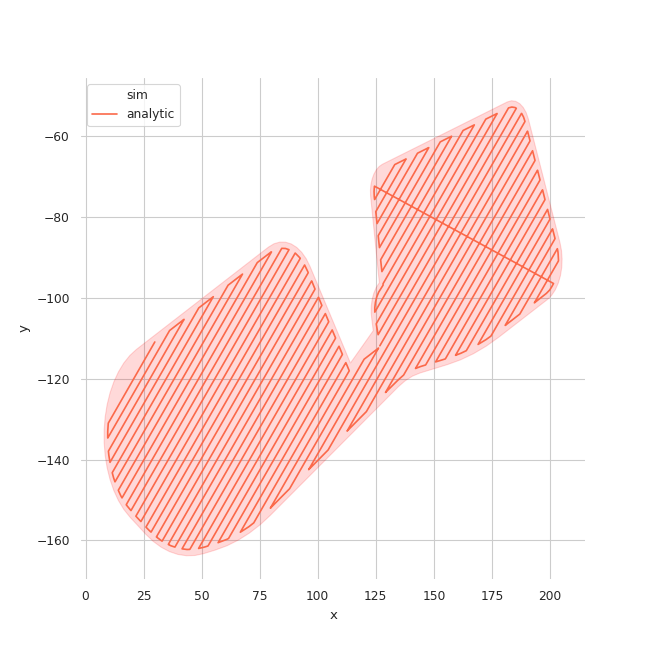
\includegraphics[width=0.333\textwidth,trim=10 10 10 10,clip]{analytic_path.png}
	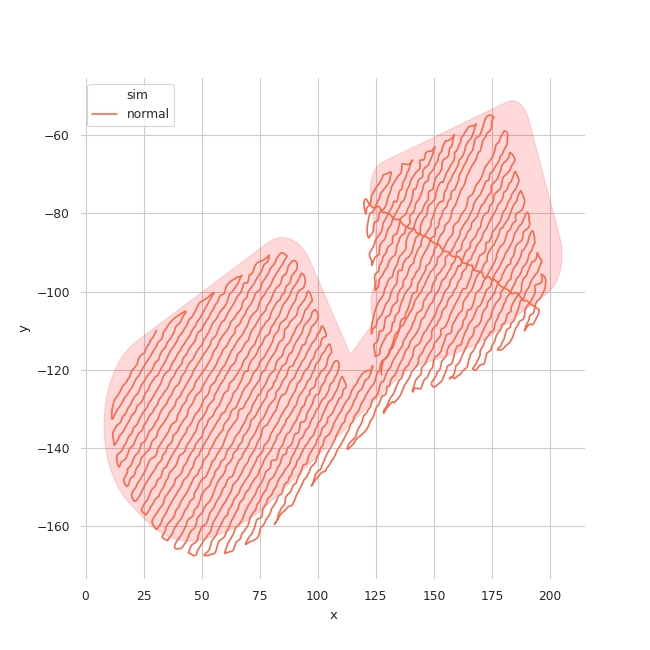
\includegraphics[width=0.333\textwidth,trim=10 10 10 10,clip]{normal_path.png}
	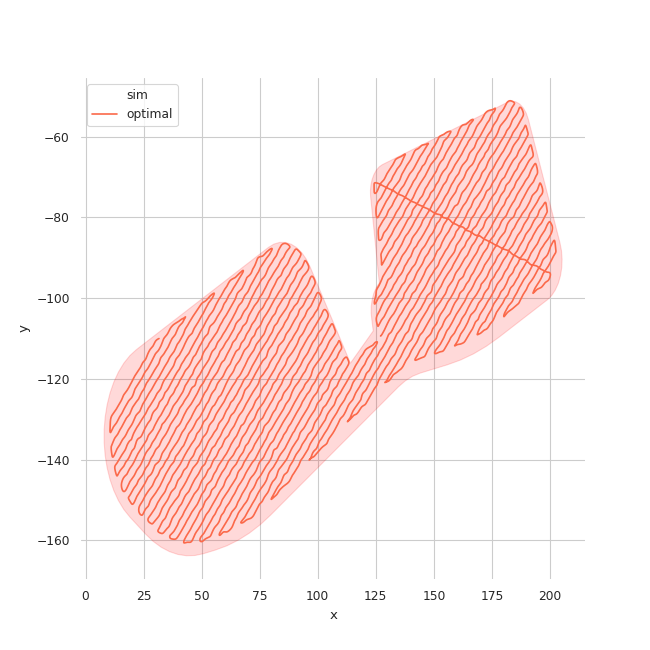
\includegraphics[width=0.333\textwidth,trim=10 10 10 10,clip]{optimal_path.png}
\end{RoyalFigure}

\begin{RoyalFigure}[!htb, label=fig:NEES_kalman]{NEES OF THE CONTROLLER}
	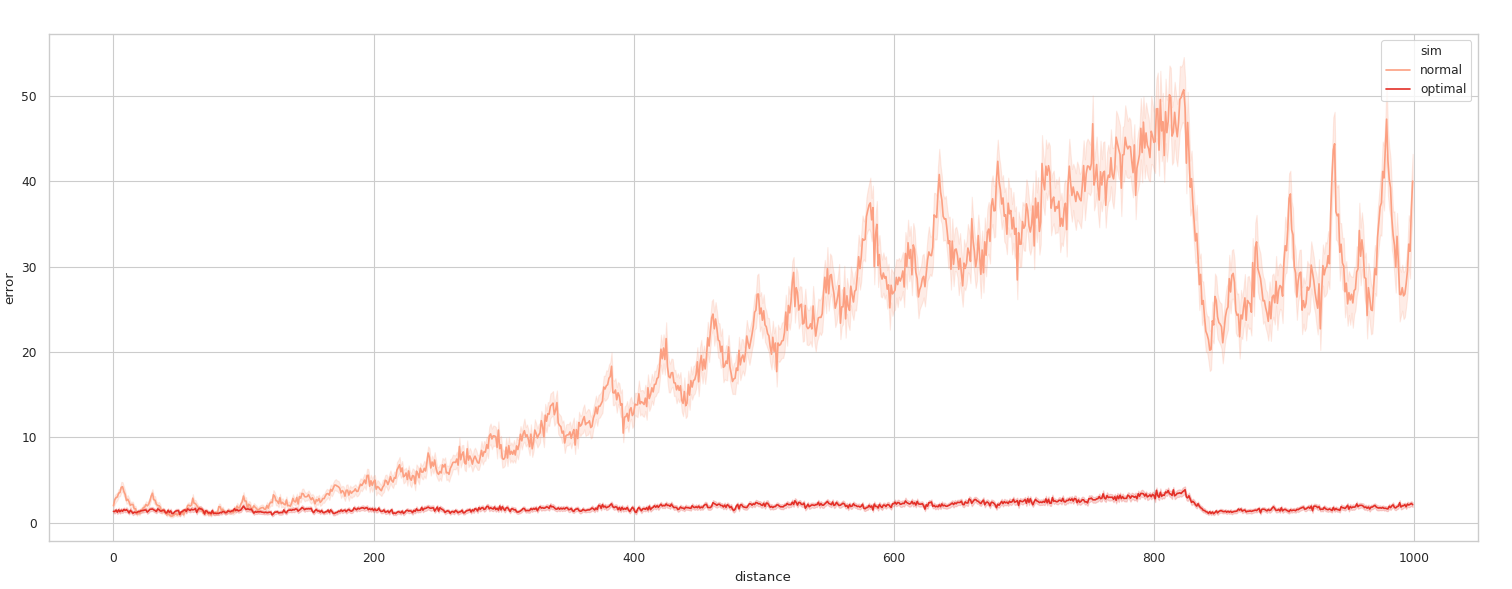
\includegraphics[width=\textwidth,trim=10 10 10 10,clip]{NEES_compared.png}
\end{RoyalFigure}
